\begin{pastexam}[label={px:df3-107-ds-02}]{地方三等資訊處理 107 年 第二題}
（申論；20 分）

給定一個權重圖（weighted graph），$G=(V, E, w)$，假設 $V = \{1, 2,\ldots,n\}$，且每個邊（edge）$e$ 的權重 $w(e)$ 都是正整數。令 $l(v)$ 為以 $v$ 為端點的所有邊中權重最小的邊。將這些邊集合起來稱作 $L$，也就是 $L = \bigcup\limits_{v\in V} l(v)$。

（每小題 5 分，共 20 分）
\begin{itemize}[leftmargin=2.2em]
\item[㈠] 假設每個邊的權重都不相同。請證明由 $L$ 中這些邊所構成的子圖（edge induced subgraph）$G[L]$ 沒有迴圈。
\item[㈡] $G[L]$ 是否一定是 $G$ 的擴張樹（spanning tree）？若是請證明之，若不一定是請給一個反例。
\item[㈢] 用以上之結論，設計一個計算 $G$ 的最小權重擴張樹（minimum spanning tree）的演算法。
\item[㈣] 在一般的應用中，邊的權重可能會相同，請修正上述之演算法，使修正後之演算法可以正確找出答案。
\end{itemize}
\end{pastexam}

\begin{pastsoln}
這題就是 Sollin（Borůvka）演算法（資結書第~24.4~節，虛擬碼~24.6）。 $G$ 是連通的簡單無向圖（要談擴張樹，$G$ 必須連通），
$n \ge 2$，每個點至少有一條邊，$l(v)$ 才有定義。

\textbf{㈠}。 \textbf{證明。} 權重都不同，所以每個點的 $l(v)$ 是唯一確定的一條邊。 假設 $G[L]$ 有迴圈 $C$，在 $C$ 上取權重
\textbf{最大}的邊 $e = \{u, v\}$（權重都不同，最大的只有一條）。 $e \in L$，所以 $e = l(u)$ 或 $e = l(v)$，不妨設 $e = l(u)$。
$u$ 在迴圈 $C$ 上，除了 $e$ 之外還有另一條 $C$ 上的邊 $e'$ 以 $u$ 為端點，而 $e$ 是 $C$ 上最重的邊，所以
$w(e') < w(e)$。 但 $l(u)$ 是以 $u$ 為端點的邊中最輕的，$w(l(u)) \le w(e') < w(e) = w(l(u))$，矛盾。 所以 $G[L]$ 沒有迴圈。
\hfill$\blacksquare$

\textbf{㈡}。 \textbf{不一定}。 $G[L]$ 沒有迴圈，但可能不連通。 反例：路徑圖 $1 - 2 - 3 - 4$，權重
$w(\{1,2\}) = 1$、$w(\{2,3\}) = 3$、$w(\{3,4\}) = 2$。
\begin{center}
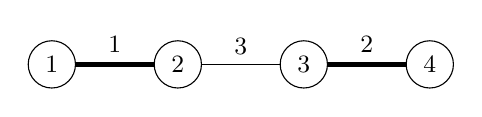
\begin{tikzpicture}[x=1.6cm,v/.style={circle,draw,minimum size=6mm,inner sep=0pt,font=\small},w/.style={font=\small,above}]
\node[v] (1) at (0,0) {1}; \node[v] (2) at (1,0) {2}; \node[v] (3) at (2,0) {3}; \node[v] (4) at (3,0) {4};
\draw[line width=1.6pt] (1)--node[w]{1}(2); \draw (2)--node[w]{3}(3); \draw[line width=1.6pt] (3)--node[w]{2}(4);
\end{tikzpicture}
\end{center}
$l(1) = l(2) = \{1,2\}$，$l(3) = l(4) = \{3,4\}$，$L = \{\{1,2\}, \{3,4\}\}$（粗線）。 $G[L]$ 只有 $2$ 條邊，有兩個連通元件
$\{1,2\}$、$\{3,4\}$，不是擴張樹（擴張樹要有 $n - 1 = 3$ 條邊、連通）。 不過 $L$ 的每一條邊都屬於最小擴張樹（下面 ㈢ 證明），
$G[L]$ 是最小擴張樹的一部分（一個森林）。

\textbf{㈢ 演算法（Borůvka／Sollin）}。 把 $L$ 的想法套在「連通元件」上反覆做：一開始每個點自成一個元件；每一回合，
每個元件挑出「一端在元件內、一端在元件外」的邊中最輕的一條，把這些邊全部加入 $T$，合併相連的元件；直到只剩一個元件。
第一回合挑出的邊正好是 $L$。
\begin{pseudo}[unbreakable]{Borůvka：權重都不同時的最小擴張樹}
\Function{MST-Boruvka}{$G, w$}
    \State $T \gets \emptyset$；每個點自成一個元件（用互斥集合記錄）
    \While{元件數 $> 1$}
        \For{每個元件 $C$}
            \State $\mathit{cheap}[C] \gets$ 離開 $C$ 的邊中權重最小的一條
        \EndFor
        \For{每個元件 $C$}
            \If{$\mathit{cheap}[C] = \{u, v\}$ 的兩端還在不同元件}
                \State $T \gets T \cup \{\{u, v\}\}$；合併 $u$、$v$ 所在的元件
            \EndIf
        \EndFor
    \EndWhile
    \State \Return $T$
\EndFunction
\end{pseudo}
\textbf{正確性}。 (1) 挑出的每條邊都安全：$\mathit{cheap}[C]$ 是跨越切割 $(C, V - C)$ 最輕的邊，由切割性質（資結書定理~24.1），
它屬於某棵最小擴張樹；權重都不同時最小擴張樹唯一（資結書定理~24.4），所以每一條挑出的邊都在\textbf{那唯一的一棵}裡，同一回合
一起加入也不會出錯。 (2) 同一回合挑出的邊不會形成迴圈：把每個元件縮成一個點，挑出的邊就是縮點圖上的「$L$」，由 ㈠ 沒有迴圈
（第 7 行檢查兩端是否已在同一元件，是為了跳過兩個元件挑到同一條邊的情形）。 (3) 只要元件數 $> 1$，$G$ 連通保證每個元件都有
離開的邊，每回合每個元件都至少和另一個合併，元件數至少減半，最多 $\lceil \log_2 n \rceil$ 回合就剩一個，$T$ 恰好 $n - 1$ 條邊。

\textbf{時間}。 每回合掃過所有邊一次找各元件的最輕邊，$O(m)$（用互斥集合查元件，近乎常數），共 $O(m \log n)$，$m = |E|$。

\textbf{㈣ 權重相同時}。 權重有相同時，㈠ 不成立，直接照做可能出錯。 例：三角形 $1, 2, 3$ 三條邊權重都是 $1$，若
$l(1) = \{1,2\}$、$l(2) = \{2,3\}$、$l(3) = \{3,1\}$（每個點在平手中各挑了不同的邊），$L$ 是整個三角形，有迴圈，加進 $T$ 就不是樹。

修正方法：\textbf{定一個一致的平手規則}，把權重相同的邊也排出唯一的先後。 比較兩條邊時用三元組
\[
\bigl(w(e),\ \min(u, v),\ \max(u, v)\bigr)
\]
依字典順序比大小：權重小的較輕；權重相同時，比較兩端編號較小的那一個；再相同就比較大的那一個。 不同的邊三元組一定不同，
所以這是一個\textbf{全序}，等於把所有權重都變成「不相同」。 演算法中所有「最小」都改用這個比較，其他不變。 這樣 ㈠ 的證明照樣
成立（把「權重最大」改成「三元組最大」），每回合不會產生迴圈；而這個全序下的最小擴張樹，用原本的權重計算總和也是最小的
（三元組的順序和原權重的順序一致，只在平手時多分先後），所以得到的是 $G$ 的一棵最小擴張樹（資結書第~24.1.7~節）。 上面三角形
的例子：$\{1,2\} < \{1,3\} < \{2,3\}$，$l(1) = \{1,2\}$、$l(2) = \{1,2\}$、$l(3) = \{1,3\}$，$L = \{\{1,2\}, \{1,3\}\}$，沒有迴圈。
\end{pastsoln}
